\section{Quicklook SCALE-LES output}
%####################################################################################

SCALE-LESモデルの出力ファイルはMPIプロセス毎に出力され,計算領域が分割された状態で出力されている.
ファイル自体のフォーマットは気候・予報(CF)メタデータ規約に対応したnetcdf4形式でアウトプットされている.
ここでは,gpviewとgradsを使用した2通りの描画方法について説明する。

\subsection{RubyDCL/Gphys: gplist, gpprint, gpview, gpvect}
%====================================================================================

Dennou系のRubyベースコマンドgpviewによって直接描画することができる.
RubyDCL/Gphysがインストールされていない場合は,Appendix \ref{sec:env_setting}を参照して
事前にインストールすること.
以下にチュートリアルで実行した結果を描画する方法についていくつか例を挙げる.


\subsubsection{ファイル内の変数を確認する}
%-----------------------------------------------------------------------------------

まず,gplistコマンドを用いてヒストリーファイル内の変数を確認する.

\begin{verbatim}
$ gplist history_d01.pe000000.nc
\end{verbatim}

\verb|history_d01.pe######.nc|のファイルはMPI並列数分だけ存在するが,
ファイルに収められている変数は基本的に同じであるため,
どれか1つのファイルについて中身を確認すればよい.
上記のコマンドを実行すると,下記のように変数リストが表示される.

{\small \begin{verbatim}
history_d01.pe000000.nc:
  x	[x=62]	'X'	(m)
  y	[y=62]	'Y'	(m)
  z	[z=36]	'Z'	(m)
  xh	[xh=62]	'X (half level)'	(m)
  yh	[yh=62]	'Y (half level)'	(m)
  zh	[zh=36]	'Z (half level)'	(m)

 ~~中略~~

  topo	[x=62,y=62]	'topography'	(m)
  lsmask	[x=62,y=62]	'fraction for land-sea mask'	(0-1)
  time	[time=24]	'time'	(seconds since 1999-01-01 00:00:00)
  time_bnds	[nv=2,time=24]	''	(seconds since 1999-01-01 00:00:00)
  DENS	[x=62,y=62,z=36,time=24]	'density'	(kg/m3)
  MOMZ	[x=62,y=62,zh=36,time=24]	'momentum z'	(kg/m2/s)
  MOMX	[xh=62,y=62,z=36,time=24]	'momentum x'	(kg/m2/s)
  MOMY	[x=62,yh=62,z=36,time=24]	'momentum y'	(kg/m2/s)
  RHOT	[x=62,y=62,z=36,time=24]	'rho * theta'	(kg/m3*K)
  QV	[x=62,y=62,z=36,time=24]	'Water Vapor mixing ratio'	(kg/kg)
  W	[x=62,y=62,z=36,time=24]	'velocity w'	(m/s)
  U	[x=62,y=62,z=36,time=24]	'velocity u'	(m/s)
  V	[x=62,y=62,z=36,time=24]	'velocity v'	(m/s)
  PT	[x=62,y=62,z=36,time=24]	'potential temp.'	(K)
  QHYD	[x=62,y=62,z=36,time=24]	'total hydrometeors'	(kg/kg)
  PRES	[x=62,y=62,z=36,time=24]	'pressure'	(Pa)
  T	[x=62,y=62,z=36,time=24]	'temperature'	(K)
  RH	[x=62,y=62,z=36,time=24]	'relative humidity'	(%)
  PREC	[x=62,y=62,time=24]	'surface precipitation rate'	(kg/m2/s)
  OLR	[x=62,y=62,time=24]	'TOA net longwave  radiation flux'	(W/m2)

 ~~中略~~
\end{verbatim} }

x, y, zなどの変数は格子情報を表しており,\verb|DENS, MOMZ, MOMX|や
\verb|PT, QHYD, PRES|といった変数が気象場のデータである.
この中から1つ,もしくは複数の変数を選んで描画する.

各気象場の変数に対してデータの軸構成が書かれている.
例えば,\verb|DENS|は空間を構成するx軸,y軸,z軸と時間を構成するtime軸によってデータが構成されている.
高度や時刻を指定して描画するためには,このようにデータを構成する軸についてあらかじめ知っておく必要がある.
例えばヒストリー出力されている時刻を調べるには次のようにコマンドを実行する.

\begin{verbatim}
$ gpprint history_d01.pe000000.nc@time
\end{verbatim}

そうすると下記のようにtime変数の値が標準出力へ表示される.

\begin{verbatim}
 1.07154e+07, 1.07172e+07, 1.0719e+07, 1.07208e+07, 1.07226e+07, 1.07244e+07,
 1.07262e+07, 1.0728e+07, 1.07298e+07, 1.07316e+07, 1.07334e+07, 1.07352e+07,
 1.0737e+07, 1.07388e+07, 1.07406e+07, 1.07424e+07, 1.07442e+07, 1.0746e+07,
 1.07478e+07, 1.07496e+07, 1.07514e+07, 1.07532e+07, 1.0755e+07, 1.07568e+07,
\end{verbatim}

SCALE-LESモデル内では日時が全て秒単位で表現されているため,ここで表記される
時刻も日時が全て秒として積算された値が時刻として表示される.
SCALE-LESモデルはデフォルト設定で,一番始めに初期値がヒストリー出力され,
そのあと\verb|HISTORY_DEFAULT_TINTERVAL|に従った時間間隔でヒストリー出力されている.
チュートリアルでは12時間積分する中で,30分ごとに出力したため,
1(初期値)+23ステップ=24ステップの時刻のデータが出力されていることがわかる.


{\small *netcdfに付属している\verb|"ncdump"|を用いてもよい.}


\subsubsection{ファイル内の変数を描画する}
%-----------------------------------------------------------------------------------

gpviewを用いて次のように描画できる.

(例 1)高度1500mにおける温度の水平分布
\begin{itemize}

\item 積分開始3時間後の様子
  \begin{verbatim}
  gpview history_d01.pe00000*@T,z=1500,time=1.07262e+07 --range=270:291 --aspect=1
  \end{verbatim}
  実行結果はFig. \ref{fig:hist_t}aのようになる(画面をクリックするか\verb|"q"|を打つことで終了する).
  オプションの\verb|z=1500,time=1.07262e+07|によって描画する高度,および時刻を指定している.
  \verb|--range=270:291|のオプションは描画する値のレンジを指定している.
  また,\verb|"--wsn=2"|のオプションを付けて実行することで,\verb|"dcl.ps"|というファイル名で
  画像をPSファイルに保存することができる.

\item 積分開始6時間後の様子:実行結果はFig. \ref{fig:hist_t}bのようになる.
  \begin{verbatim}
  gpview history_d01.pe00000*@T,z=1500,time=1.0737e+07 --range=270:291 --aspect=1
  \end{verbatim}
  先との変更点はtimeオプションの引数だけである.

\item 積分開始9時間後の様子:実行結果はFig. \ref{fig:hist_t}cのようになる.
  \begin{verbatim}
  gpview history_d01.pe00000*@T,z=1500,time=1.07478e+07 --range=270:291 --aspect=1
  \end{verbatim}

\end{itemize}


\begin{figure}[t]
\begin{center}
  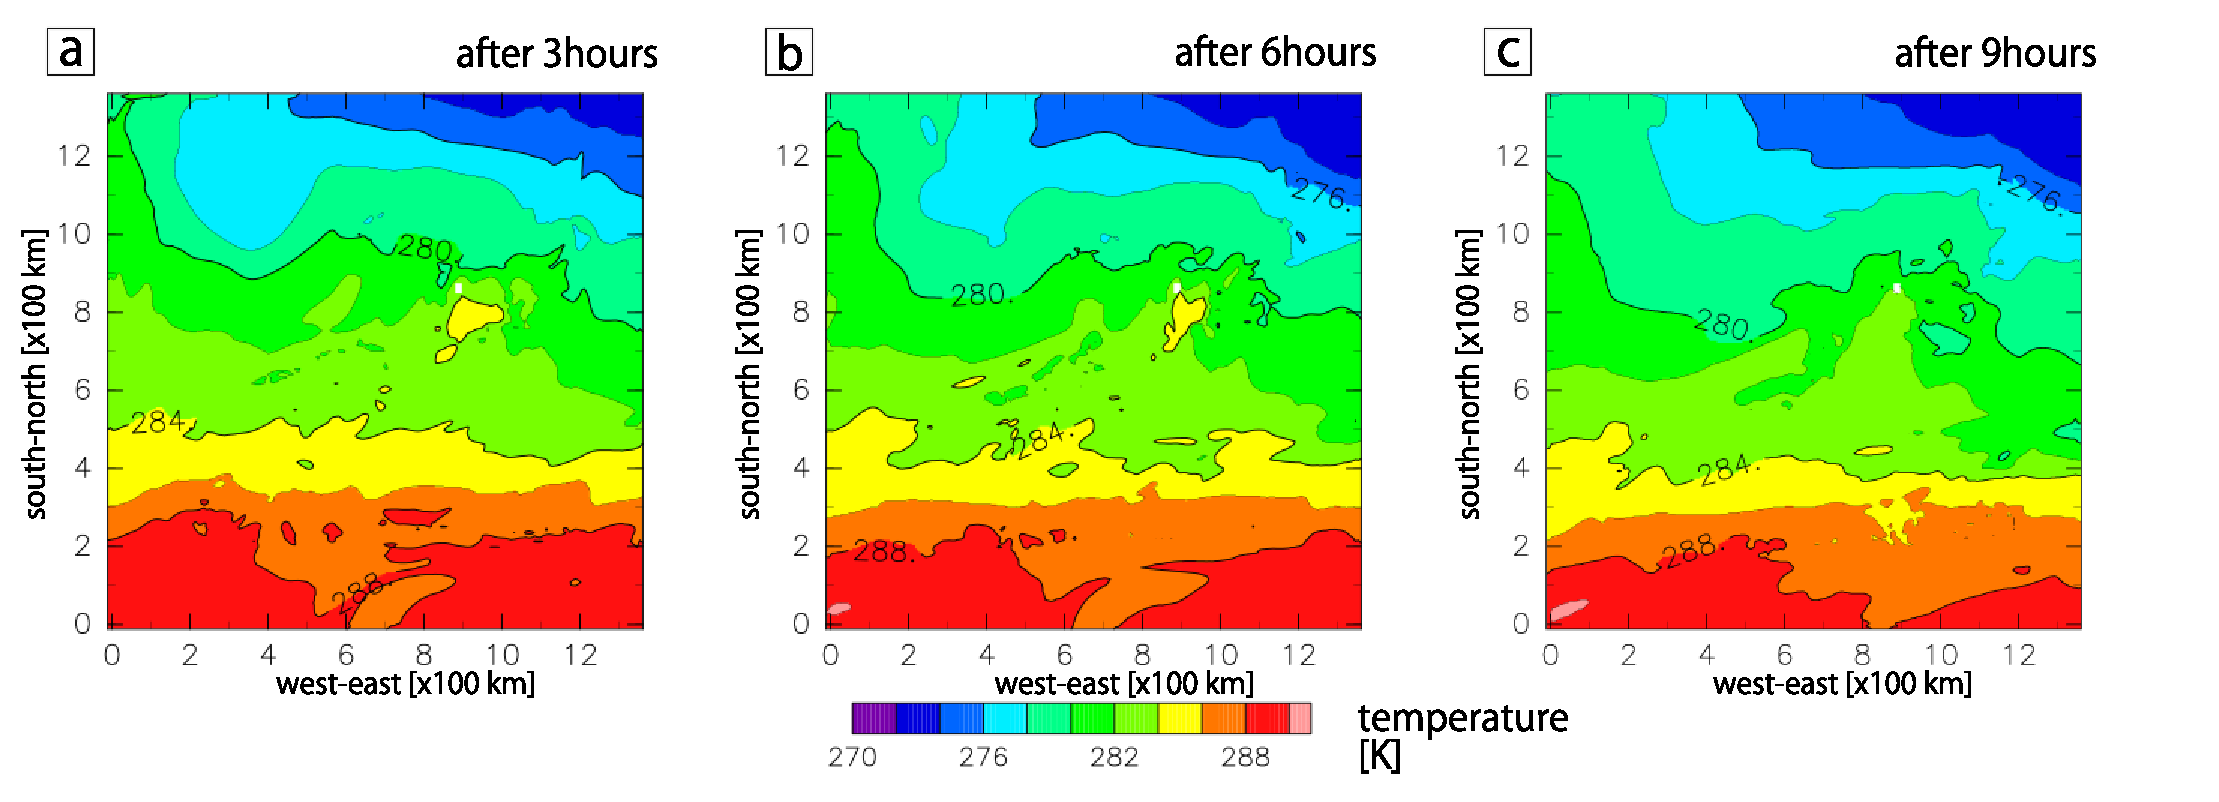
\includegraphics[width=0.9\hsize]{./figure/gpview_hist_t.eps}\\
  \caption{高度1.5kmにおける気温の分布}
  \label{fig:hist_t}
\end{center}
\end{figure}


(例 2)高度1500mにおける相対湿度と水平風の分布
\begin{itemize}

\item 積分開始3時間後の様子
  \begin{verbatim}
  gpvect --scalar --slice z=1500,time=1.07262e+07 --nocont --range=10:102        \
         --aspect=1 --xintv=10 --yintv=10 --unit_vect history_d01.pe00000*@RH    \
         history_d01.pe00000*@U history_d01.pe00000*@V
  \end{verbatim}
  実行結果はFig. \ref{fig:hist_rh}aのようになる.
  ここでは\verb|gpview|ではなくベクトルを描画することができる\verb|gpvect|を使用して描画する.
  オプションの\verb|--xintv=10 --yintv=10|は,ベクトルを描画する格子点間隔を指定している.

\item 積分開始6時間後の様子:実行結果はFig. \ref{fig:hist_rh}bのようになる.
  \begin{verbatim}
  gpvect --scalar --slice z=1500,time=1.0737e+07 --nocont --range=10:102        \
         --aspect=1 --xintv=10 --yintv=10 --unit_vect history_d01.pe00000*@RH    \
         history_d01.pe00000*@U history_d01.pe00000*@V
  \end{verbatim}

\item 積分開始9時間後の様子:実行結果はFig. \ref{fig:hist_rh}cのようになる.
  \begin{verbatim}
  gpvect --scalar --slice z=1500,time=1.07478e+07 --nocont --range=10:102        \
         --aspect=1 --xintv=10 --yintv=10 --unit_vect history_d01.pe00000*@RH    \
         history_d01.pe00000*@U history_d01.pe00000*@V
  \end{verbatim}
\end{itemize}


\begin{figure}[t]
\begin{center}
  \includegraphics[width=0.9\hsize]{./figure/gpview_hist_rh.eps}\\
  \caption{高度1.5kmにおける相対湿度と水平風の分布:カラーシェードは相対湿度,ベクトルは水平風を示す}
  \label{fig:hist_rh}
\end{center}
\end{figure}


(例 3)QHYD(凝結物の混合比)についての計算領域西端から800kmの地点における鉛直-南北断面図

\begin{verbatim}
gpview history_d01.pe00000*@QHYD,x=800000,y=100000:600000,z=0:16000,time=1.0737e+07
\end{verbatim}
積分開始6時間後の様子で,実行結果はFig. \ref{fig:hist_qhyd}のようになる.
オプションの\verb|x=800000,y=100000:600000,z=0:16000|によって,xは800kmの地点,
yは100kmから600kmの範囲,zは0kmから16kmの範囲を描画するように指定している.


その他の描画例を下記に挙げる.
\begin{itemize}

\item 水平風南北成分を描画する:\\
  高度1000m指定,カンバスの縦横比=1,コンターなし,変数の描画範囲=4.8~5.2 [m/s],
  時間軸をアニメーション(クリックで進む)\\
  \verb|$ gpview history.pe00*@V,z=1000 --aspect 1 --nocont --range=4.8:5.2 --anim time|

\item 水蒸気混合比の南北-鉛直断面図を描画する:\\
  東西方向に50kmの位置を指定,コンターなし,時間軸をアニメーション,\verb|"--Gaw"|のオプションに
 より自動でアニメが進む,横軸と縦軸を交換 (exch)\\
  \verb|$ gpview history.pe00*@QV,x=50000 --aspect 1 --nocont --anim time --Gaw --exch|

\end{itemize}


\begin{figure}[t]
\begin{center}
  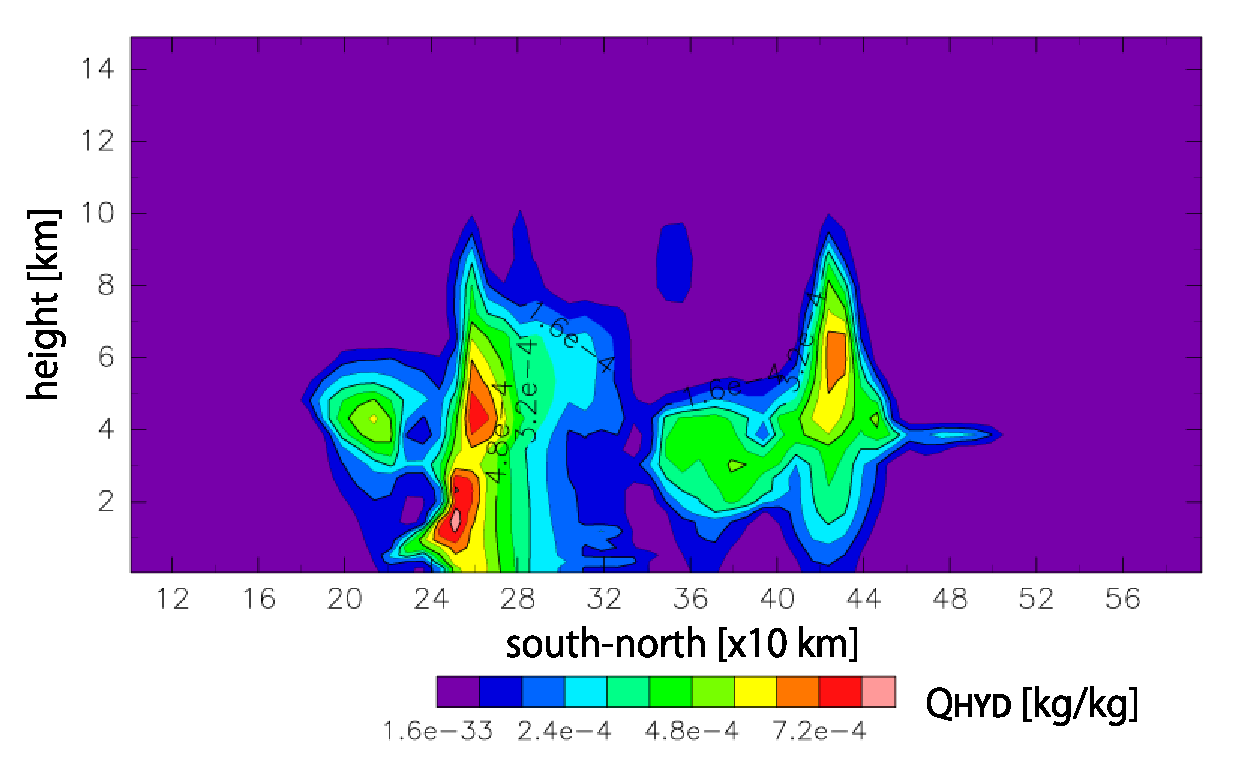
\includegraphics[width=0.7\hsize]{./figure/gpview_hist_qhyd.eps}\\
  \caption{x=800kmにおける鉛直-南北断面図}
  \label{fig:hist_qhyd}
\end{center}
\end{figure}


また,チュートリアルの中でも使用してきたが,下記のように\verb|init_****.pe#####.nc|ファイルなどを
指定することで,初期値・境界値や下端境界条件のファイルの中身も見ることが出来る.

\begin{itemize}
 \item \verb|$ gpview init_00000000000.000.pe00*@MOMX,z=1000 --aspect 1 --nocont|
 \item \verb|$ gpview boundary.pe00*@VELX,z=1000 --nocont --anim time|
 \item \verb|$ gpview topo.pe00*@TOPO --aspect 1|
 \item \verb|$ gpview landuse.pe00*@FRAC_LAND --aspect 1|
\end{itemize}


その他のオプション等については--helpを使ってヘルプを表示させるか,電脳倶楽部のWebページ
(\url{http://ruby.gfd-dennou.org/products/gphys/doc/gpview.html})を参照すること.

